
% One chapter ---------------------------------------------------------
\chapter*{One}
\addcontentsline{toc}{chapter}{One}

\begin{flushright}
\parbox{0.8\textwidth}{
\emph{God is not external to anyone, but is present with all things, though
they are ignorant that he is so. \\
\hspace*{\fill}{\textperiodcentered \textperiodcentered \textperiodcentered \hspace*{0.2em} Plotinus} } }
\end{flushright}

\noindent
One is chess variant which is played on 26 x 26 board, with white
and darker violet fields, with light purple and fuchsia pieces.
Star colors are the same as for ordinary pieces, i.e. light purple and
fuchsia. In algebraic notation, columns are enumerated from 'a' to 'z',
and rows are enumerated from '1' to '26'. A new piece is introduced,
Starchild.

\textbf{\huge{TODO :: Star colors !!!}} % TODO :: FIX ME !!!

\clearpage % ..........................................................

\section*{Starchild}
\addcontentsline{toc}{section}{Starchild}

\noindent
\begin{wrapfigure}{l}{0.4\textwidth}
\centering
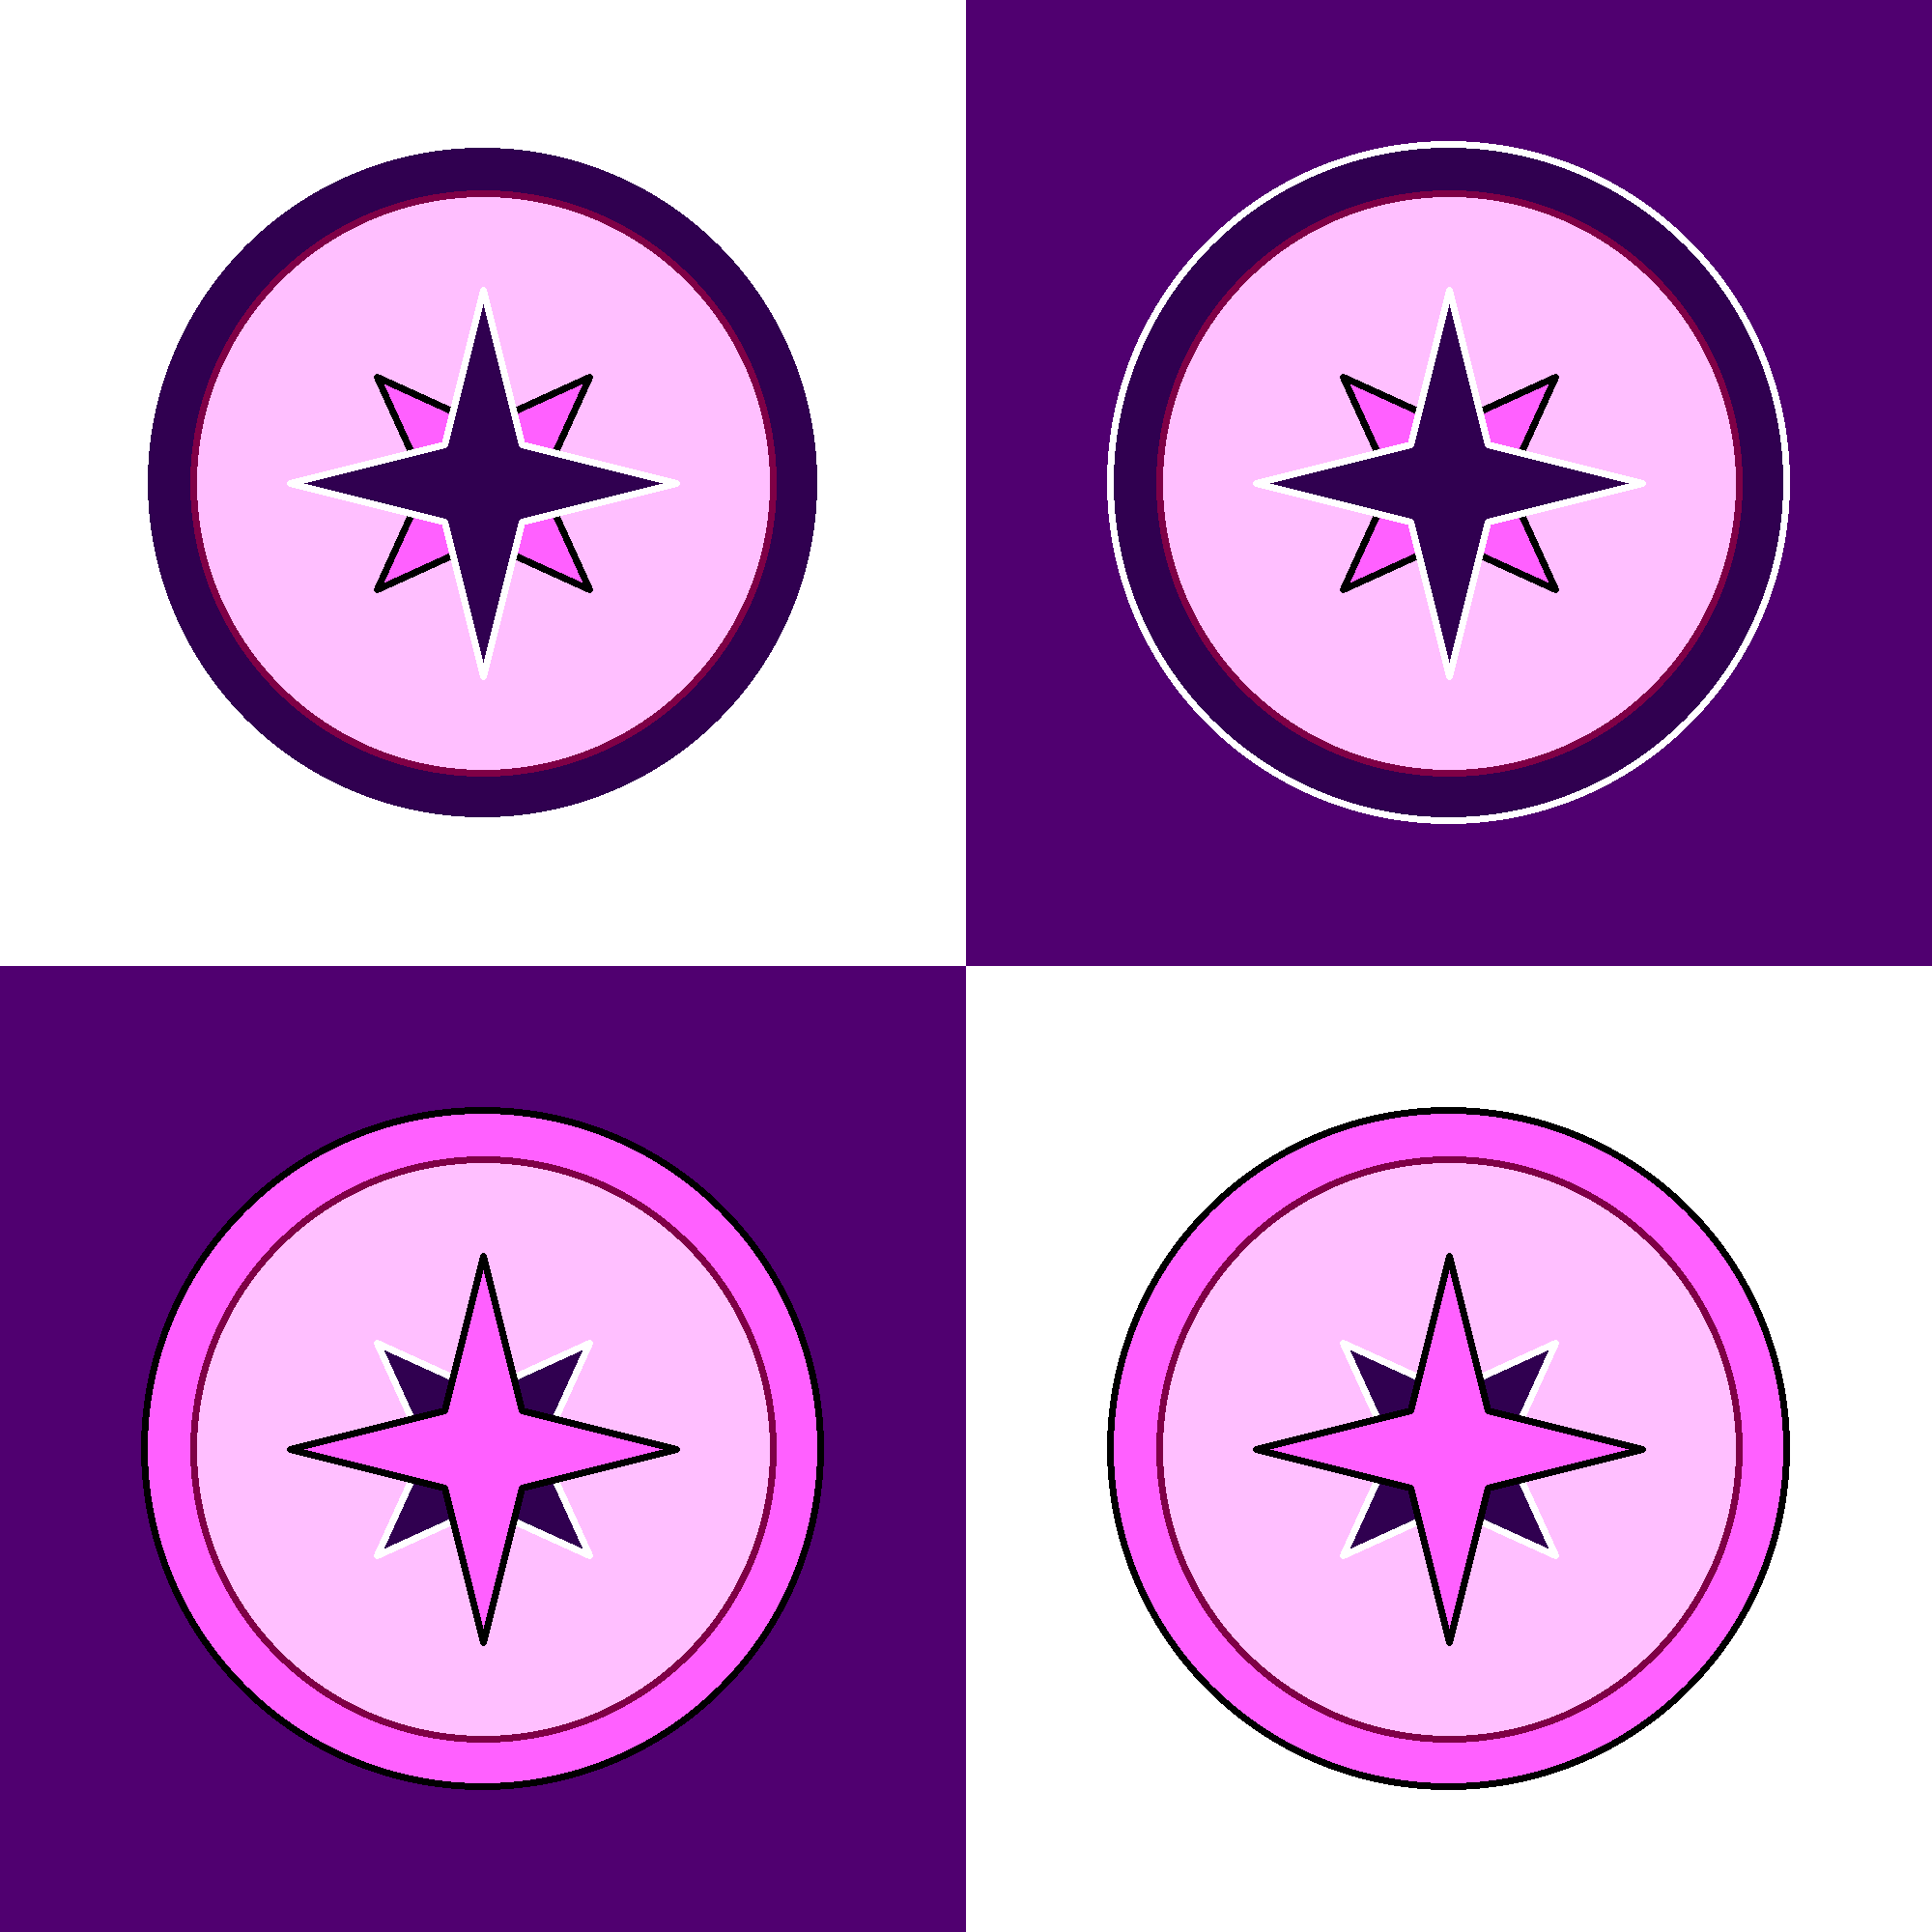
\includegraphics[width=0.4\textwidth, keepaspectratio=true]{pieces/16_starchild.png}
\caption{Starchild}
\label{fig:16_starchild}
\end{wrapfigure}

Starchild cannot be converted, but can be activated.

[?] Starchild does accumulate momentum, but does not spend it while moving. [?]

\clearpage % ..........................................................

\section*{Initial setup}
\addcontentsline{toc}{section}{Initial setup}

Initial setup can be seen in image below:

\noindent
% \begin{figure}[t]
\begin{figure}[h]
\includegraphics[width=1.0\textwidth, keepaspectratio=true]{boards/22_one.png}
\caption{One board}
\label{fig:22_one}
% \centering
\end{figure}

\clearpage % ..........................................................
% --------------------------------------------------------- One chapter
